\documentclass{article}
\usepackage[utf8]{inputenc}
\usepackage[margin=1in]{geometry}

\title{480 - Homework 5}
\author{Victor Zhang}
\date{November 1, 2021}

\usepackage[utf8]{inputenc}
\usepackage{amsmath}
\usepackage{amsfonts}
\usepackage{natbib}
\usepackage{graphicx}
% \usepackage{changepage}
\usepackage{amssymb}
\usepackage{xfrac}
% \usepackage{bm}
% \usepackage{empheq}
\usepackage{subcaption}
\usepackage{hyperref}
\usepackage{cleveref}

\newcommand{\contra}{\raisebox{\depth}{\#}}

\newenvironment{myindentpar}[1]
  {\begin{list}{}
          {
            \setlength{\leftmargin}{#1}
            \setlength{\rightmargin}{#1}
          }
          \item[]
  }
  {\end{list}}

\pagestyle{empty}
\hypersetup{
  colorlinks=true,
  linkcolor=blue,
}

\begin{document}

\maketitle
% \begin{center}
% {\huge Econ 482 \hspace{0.5cm} HW 3}\
% {\Large \textbf{Victor Zhang}}\
% {\Large February 18, 2020}
% \end{center}

\section{}
Suppose Eva assigns $Pr(R) = r, Pr(B) = b, Pr(y) = y$. According to EU theory,
\begin{gather*}
r \cdot u(10) > (b + y) \cdot u(5)\\
b \cdot u(10) > (r + y) \cdot u(5)\\
b \cdot u(10) = y \cdot u(10)
\end{gather*}
So Eva must assign $b = y$ and we may rewrite the constraints as
\begin{gather}
r \cdot u(10) > 2b \cdot u(5)\\
b \cdot u(10) > (r + b) \cdot u(5)
\end{gather}

\subsection{}
If Eva is risk-averse, her utility function is concave and $u(10) < 2 u(5)$. So for (1) to hold, $r > b$. But by concavity,
$$b \cdot u(10) < 2b \cdot u(5) < (r + b) \cdot u(5)$$
a contradiction $\contra$

\subsection{}
This is possible. Suppose $u(x) = x^2$ and $r = b = y = \frac{1}{3}$. Then both equations (1) and (2) are satisfied $\Box$

\section{}
\subsection{}
See Figure~\ref{fig:fig1}.
\begin{figure}[ht!]
\begin{subfigure}[h]{0.45\linewidth}
  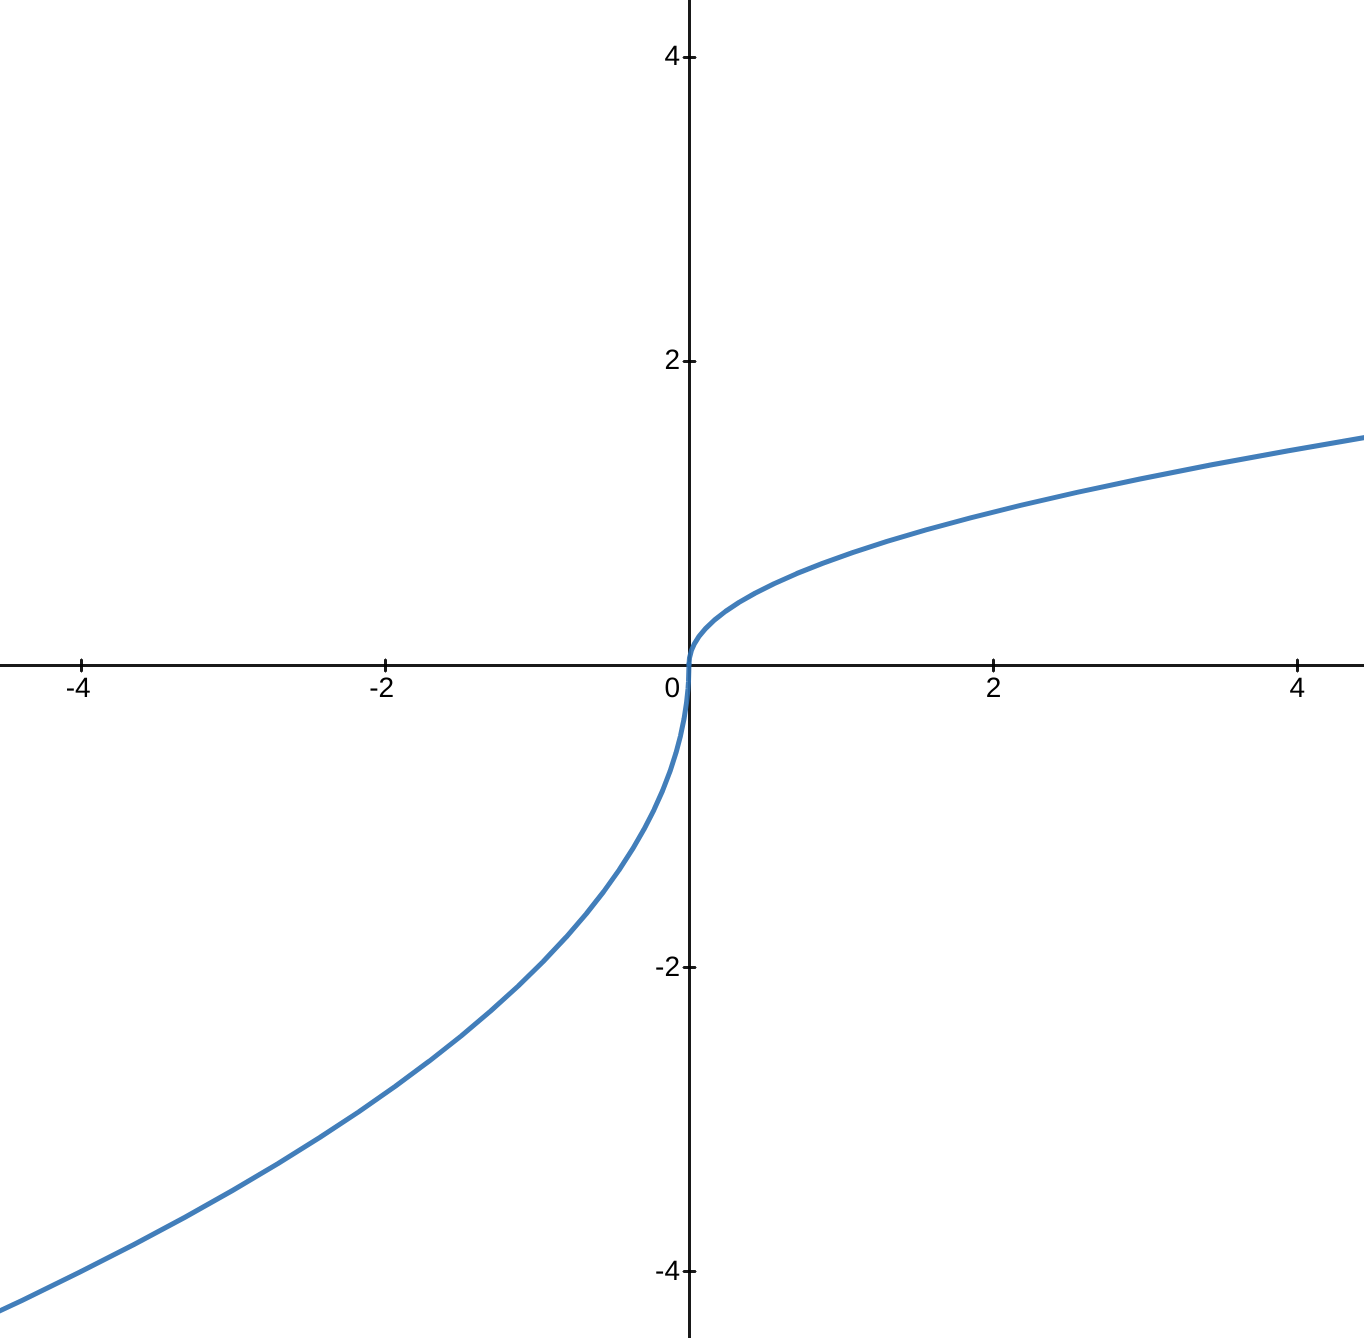
\includegraphics[width=\linewidth]{img/hw_5_1.png}
  \caption{$v(x)$}
\end{subfigure}
\hfill
\begin{subfigure}[h]{0.45\linewidth}
  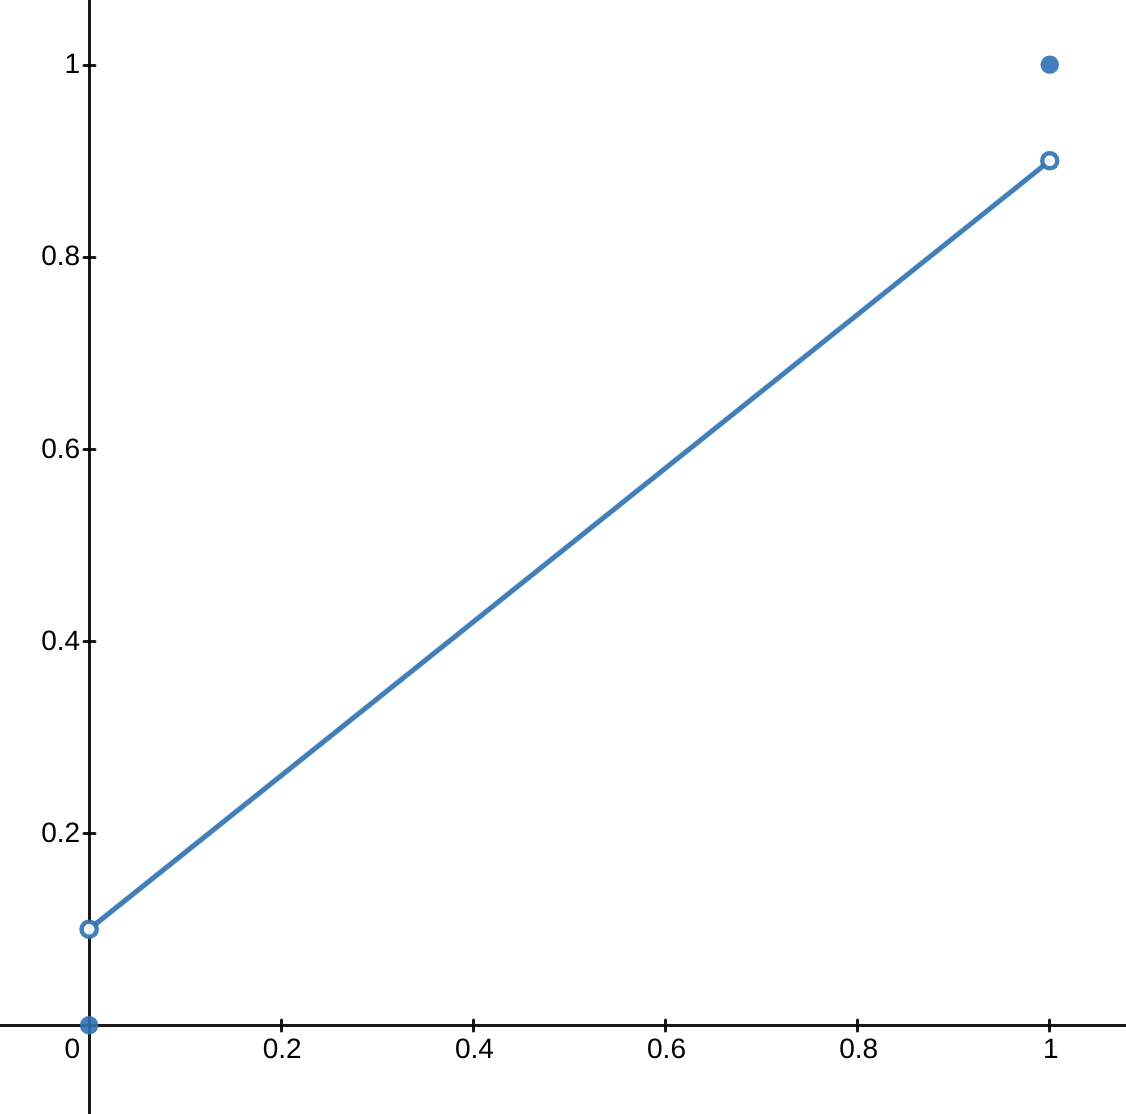
\includegraphics[width=\linewidth]{img/hw_5_2.png}
  \caption{$\pi(p)$}
\end{subfigure}
\caption{}
\label{fig:fig1}
\end{figure}
\subsection{}
The value of option S is
$$\pi(1) \sqrt{2/2} = 1$$
The value of option G is
$$\pi(0.6)\sqrt{4/2} = 0.82$$
So Pooh will choose the sure option $\Box$

\subsection{}
The value of option S is
$$\pi(1) (-2\sqrt{2}) = -2.828$$
The value of option G is
$$\pi(0.4) (-2\sqrt{4}) = -1.68$$
so Eeyore will choose the gamble $\Box$

\section{}
Her expected values are
\begin{gather*}
V(A) = (\frac{2}{3} 0.7 + \frac{1}{30})v(-800) = \frac{1}{2} v(-800)\\
V(B) = v(-400)
\end{gather*}
By prospect theory, $v$ is convex on negative domain so $\frac{1}{2} v(-800) > v(-400)$ and we may predict Susan will choose lottery A $\Box$

\end{document}

% List of tex snippets:
%   - tex-header (this)
%   - R      --> \mathbb{R}
%   - Z      --> \mathbb{Z}
%   - B      --> \mathcal{B}
%   - E      --> \mathcal{E}
%   - M      --> \mathcal{M}
%   - m      --> \mathfrak{m}({#1})
%   - normlp --> \norm{{#1}}_{L^{{#2}}}
